\documentclass[a4paper]{article}
\usepackage{fullpage}
\usepackage{amsmath}
\usepackage{pdfpages}
\usepackage{booktabs}

\begin{document}
\counterwithout{equation}{section}

\title{Praktikumsbericht \\ Physikalisches Praktikum \\ Versuch: T5 \\ Thermoelement und Newtonsches Abkühlungsgesetz}
\author{Janosch Ehlers, Raul Renken}
\date{Vom: Do, 11.04.19 }
\maketitle
\newpage

\section*{0.0 Inhalt}
\begin{itemize}
\item[0.0] Inhalt
\item[1.0] Ziel des Versuchs
\item[2.0] Theoretischer Hintergrund
\begin{itemize}
\item[2.1] 		Thermoelektrische Temperaturmessung
\item[2.2] 		Newtonsches Abkühlungsgesetz
\end{itemize}
\item[3.0] Versuchsaufbau und -durchführung
\item[4.0] Auswertung
\begin{itemize}
\item[4.1] 		Bestimmung des Seebeck-Koeffizienten
\item[4.2] 		Temperaturverlauf der Abkühlung einer Wachsprobe
\item[4.3] 		Überprüfung des newtonschen Abkühlungsgesetzes
\item[4.4] 		Vergleich empirischer Werte mit der Theorie
\item[4.5] 		Zusammenfassung
\end{itemize}
\end{itemize}

\section*{1.0 Ziel des Versuchs}

Unter Verwendung eines Thermoelements, wird das Verhalten verschiedener Stoffe hinsichtlich ihrer Temperatur, beim Abkühlen untersucht. Beobachtet wird dabei auch der Einfluss von Masse und Oberfläche. Es wird außerdem der Vergleich zwischen empirischen Daten und dem newtonschen Abkühlungsgesetz diskutiert.\\

\section*{2. Theoretischer Hintergrund}
\subsection*{2.1 Thermoelektrische Temperaturmessung}
Die Messmethode, welche in diesem Versuch verwendet wurde, beruht auf dem thermoelektrischen Effekt. Indem Zwei unterschiedliche Metalle an Zwei die Messmethode, welche in diesem Versuch verwendet wurde, beruht auf dem thermoelektrischen Effekt. Indem Zwei unterschiedliche Metalle an Zwei Stellen mit einander verlötet sind, wird ein Leiterkreis gebildet. Die Leiterelektronen beider Metalle besitzen, aufgrund der verschiedenen Elektronenkonfigurationen, eine unterschiedliche Austrittsarbeit. Werden die Metalle, wie oben beschrieben, zusammengefügt, entsteht ein Potenzial, welches durch eine Elektronenübertragung von dem Metall mit geringerer Austrittsarbeit zu dem Metall mit höherer Austrittsarbeit, ausgeglichen werden kann. Dadurch werden die Metalle Positiv oder Negativ geladen. Die Abhängigkeit zwischen Austrittsarbeit und Temperatur ist Werkstoffspezifisch.stellen mit einander verlötet sind, wird ein Leiterkreis gebildet. Die Leiterelektronen beider Metalle besitzen, aufgrund der verschiedenen Elektronenkonfigurationen, eine unterschiedliche Austrittsarbeit. Werden die Metalle, wie oben beschrieben, zusammengefügt, entsteht ein Potential, welches durch eine Elektronenübertragung von dem Metall mit geringerer Austrittsarbeit zu dem Metall mit höherer Austrittsarbeit, ausgeglichen werden kann. Dadurch werden die Metalle Positiv oder Negativ geladen. Die Abhängigkeit zwischen Austrittsarbeit und Temperatur ist Werkstoffspezifisch. Da Zwei verschiedene Metalle verwendet werden, verändert sich die Kontaktspannung zwischen den Metallen mit der Temperatur. Haben nun beide Lötstellen die gleiche Temperatur, heben sich die Kontaktspannungen gegenseitig auf. Erzeugen wir eine Temperatur Differenz zwischen den beiden Lötstellen, entsteht eine sogenannte Thermospannung: $U_T$. Da die Thermospannung proportional zur Temperaturdifferenz zwischen den Kontaktstellen der Metalle, für $T\in [273;373]K$, ist, kann mit einer Referenztemperatur an der einen Kontaktstelle eine Temperaturmessung relativ zur Referenztemperatur ermittelt werden. Der Proportionalitätskoeffizient ist hierbei der sogenannte Seebeck Koeffizient, welcher über (1) definiert ist. 
\begin{align}  
S = \frac{dU_T}{dT}
\end{align}
Hierbei ist $s$ Der Seebeck Koeffizient, Während $dU_T$ Die Kontaktspannungsdifferenz ist und $dT$ die Temperaturdifferenz zwischen den Kontaktstellen darstellt. Im folgenden kann die Temperatur in dem gegebenen Intervall mit Gleichung (2) berechnet werden:
\begin{align}
dT=\frac{\Delta U}{S}
\end{align}

\subsection*{2.2 Newtonsches Abkühlungsgesetz}
Gibt ein Körper Wärme an seine Umgebung ab, ist die Menge der abgegebenen Wärme ($\delta Q$) proportional zu der Differenz zwischen Eigentemperatur ($T$) und Umgebungstemperatur ($T_U$)	, sowie Oberfläche ($df$) und Zeit ($dt$). Definiert ist dies über: 
\begin{align}
\delta Q=-\alpha(T-T_U)\cdot df\cdot dt
\end{align}
Durch Integration, Einführung der Wärmekapazität und Umstellen erhalten wir: 
\begin{align}
T(t)-T_U&=(T_{(t=0)}-T_U)\cdot e^{\frac{-t}{\tau}}\\
\tau&=\frac{C}{\overline{\alpha}F}
\end{align}
Dies ist nun eine exponential Funktion, mit dessen Hilfe wir nun präzise Vorhersagen zum Temperaturverlauf treffen können. Suchen wir hingegen $\tau$ so lässt sich die Gleichung nach Gleichung (6) Umstellen:
\begin{align}
\tau=\frac{-t}{\ln\left(\frac{T(t)-T_U}{T_0-T_U}\right)}
\end{align}

\newpage
\section*{3.0 Versuchsaufbau und -durchführung}
Um Gleichung (6) experimentell nachzuweisen wurde folgender Versuchsaufbau verwendet: Zwei unterschiedliche Metallstäbe wurden an Ihren enden zusammen gelötet. Und so verbogen das die Lötstellen in Bechergläser getaucht werden können. Eines der Metallstäbe wurde geteilt und ein Spannungsmessgerät wurde dazwischen geschaltet. Das Thermoelement wurde nun durch siedendes Wasser auf der einen und Eiswasser auf der anderen Seite geeicht, indem hier der Seebeck Koeffizient mit $dT=100K$ ermittelt wurde. Dadurch wurde sichergestellt, das etwaige Fehler/Ungenauigkeiten im Aufbau durch diesen Koeffizienten, bei der Auswertung herausgerechnet werden. In einem ersten Versuch wurde die Temperatur einer flüssigen Stearinsäure-Phase beim Erstarren beobachtet. Die Stearinsäure wurde in einem Reagenzglas zum Schmelzen gebracht. Danach wurde eine der Lötstellen in das Reagenzglas getaucht. Die andere Lötstelle wurde weiterhin mit dem Eiswasser gekühlt. Die Kühlung mit Eiswasser an der zweiten Lötstelle wurde für alle folgenden Versuche beibehalten, um eine Referenztemperatur aufrecht zu erhalten. Das Wachs wurde dann im folgenden mit $(288\pm 0,46)K$ warmen Wasser gekühlt. Ab diesem Zeitpunkt wurden alle $15s$ die angezeigte Spannung festgehalten, bis kein signifikante Änderung der Spannung zu erkennen war. In einem zweiten Versuch wurden zwei Messing Blöcke auf $~593K$ erhitzt. Diese Temperatur wurde abgeschätzt und der Versuch wurde gestartet in dem Moment, indem das Metallstück zu glühen begann. Beide Metallstücke hatten eine kleine Öffnung, in die die Lötstelle des Thermoelements eingeführt werden konnte. So konnte die Temperatur beim Abkühlen ermittelt werden. Um den Prozess zu beschleunigen, wurde ein Lüfter installiert, um den Luftstrom an der Oberfläche des Körpers zu erhöhen.
\newpage
\section*{4. Auswertung}
\subsection*{4.1 Bestimmung des Seebeck-Koeffizienten}
Zur Bestimmung des Seebeck-Koeffizienten wird eine der Lötstellen des Thermoelements in ein Becherglas mit Eiswasser von $273K$ getaucht, während die andere in ein Becherglas mit siedendem Wasser von $373K$ getaucht wird. Die für diese Temperaturdifferenz von $\Delta T=(100\pm 2)K$ gemessene Spannung zwischen den beiden Lötstellen beträgt $U=(2,89\pm 0,01)mV$. Gemäß des Versuchsskripts gilt, in dem in diesem Versuch betrachteten Temperaturbereich: $T\in [273;573]K$, ein linearer Zusammenhang zwischen Spannung und Temperatur. Daher ergibt sich nach Gleichung (1) für den Seebeck-Koeffizienten:
\begin{align}
S=\frac{2,89mV}{100K}
\end{align}
Der relative Größtfehler wird nach Gleichung (8) berechnet:
\begin{align}
\frac{\Delta S}{S}=\sqrt{\frac{\Delta U}{U}+\frac{\Delta T}{T}}
\end{align}
Für den Absoluten Fehler des Seebeck-Koeffizienten ergibt sich also:
\begin{align}
\Delta S=S\cdot \sqrt{\left(\frac{0,00001V}{0,00289V}\right)^2+\left(\frac{2K}{100K}\right)^2}=0,02029711893\frac{V}{K}\cdot 0,00289\frac{V}{K}=0,000058659\frac{V}{K}\approx 5,87\ E-5
\end{align}
\begin{align}
S=(0,00289\pm 5,87\ E-5)\frac{V}{K}
\end{align}
\subsection*{4.2 Temperaturverlauf der Abkühlung einer Wachsprobe}
Es soll der Temperaturverlauf der Abkühlung einer Wachsprobe (Stearinsäure) bestimmt und anhand der aufgenommenen Werte die Erstarrungstemperatur des Wachses ermittelt werden. Es ist zu erwarten, dass die Temperatur bei erreichen der Erstarrungstemperatur über einen längeren Zeitraum konstant bleibt. Dies ist damit zu begründen, dass zunächst nur Wärme an die Umgebung abgegeben wird, die durch den Übergang vom flüssigen in den festen Aggregatzustand frei wird. Erst wenn das Wachs vollständig erstarrt ist, nimmt dessen Temperatur weiter ab. Um den Temperaturverlauf aufzunehmen wurde eine Wachsprobe geschmolzen und eine der Lötstellen des Thermoelements hinein getaucht. Die aufgenommenen Spannungen können der Tabelle 1 entnommen werden. Der Messfehler ergibt sich über Gleichung (11):
\begin{align}
\Delta T=T\cdot\sqrt{\left(\frac{\Delta U}{U}\right)^2+S^2}
\end{align}
\begin{center}
\begin{tabular}{ccc}
Spannung ($mV$) & Temperatur ($K$)\footnotemark & Größtfehler d. Temp. ($\pm K$)\\
\hline
1,49 & 51,56 & 1,1\\
1,53 & 52,94 & 1,13\\
1,70 & 58,82 & 1,24\\
2,64 & 91,35 & 1,89\\
2,47 & 85,47 & 1,77\\
2,32 & 80,28 & 1,67\\
2,20 & 76,12 & 1,58\\
2,11 & 73,01 & 1,52\\
2,02 & 69,90 & 1,46\\
1,97 & 68,17 & 1,43\\
1,96 & 67,82 & 1,42\\
1,94 & 67,13 & 1,41\\
1,93 & 66,78 & 1,4\\
1,93 & 66,78 & 1,4\\
1,93 & 66,78 & 1,4\\
1,93 & 66,78 & 1,4\\
1,93 & 66,78 & 1,4\\
\end{tabular}
\end{center}
\begin{flushleft}
\small Tabelle 1: Zeitlicher Temperaturverlauf der Wachsprobe
\end{flushleft}
\footnotetext{Relativ zur Referenztemperatur von $273K$. Es wird davon Ausgegangen, dass diese über das Gesamte Experiment Konstant blieb.}
Die in Tabelle 1 aufgeführten Messwerte sind in der Abb. 1 aufgetragen. Dabei werden die Fehler der einzelnen Werte nicht berücksichtigt, da sie zu gering sind um sie in Form von Fehlerbalken ein zu Zeichen. Die Temperatur fällt zunächst exponentiell ab, was einem Temperaturverlauf gemäß des newtonschen Abkühlungsgesetzes entspricht. Wie erwartet bleibt die Temperatur daraufhin für einen längeren Zeitraum bei $(339,78\pm 1,4)K$ konstant. Bei dieser Temperatur handelt es sich demnach um die Erstarrungstemperatur. Der Literaturwert für die Erstarrungstemperatur der Stearinsäure liegt bei $342K$\footnote{http://www.chemie.de/lexikon/Stearins\%C3\%A4ure.html} und weicht somit auch unter Berücksichtigung des Fehlers von dem im Versuch bestimmten Wert ab. Dennoch liegt der im Versuch bestimmte Wert für die Erstarrungstemperatur relativ nah am Literaturwert. Die Abweichung könnte möglicherweise auf Verunreinigungen der im Versuch verwendeten Stearinsäure zurückzuführen sein. Weiterhin könnte die Temperatur des verwendeten Vergleichsmediums von $273K$ abweichen und somit die Messung verfälschen. Es fällt auf, dass die Temperatur der Wachsprobe zunächst ansteigt, bevor sie fällt. Dies ist auf einen Messfehler zurückzuführen. Die Messung wurde begonnen, bevor die Lötstelle die Temperatur des umgebenden Wachses angenommen hat, wodurch zunächst ein Temperatur anstieg verzeichnet wird. Dabei handelt es sich jedoch nur um eine verzögerte Reaktion des Thermoelements. Idealerweise sollte die Messung erst bei erreichen der maximalen Temperatur begonnen werden. 
\subsection*{4.3 Überprüfung des newtonschen Abkühlungsgesetzes}
Zur Überprüfung des newtonschen Abkühlungsgesetzes werden zwei Messingkörper gleicher Masse aber verschiedener Oberfläche stark erhitzt. Für beide Körper wird alle 30 Sekunden die Spannung zwischen beiden Lötstellen aufgenommen und so der Temperaturverlauf beobachtet. Während der gesamten Messung wird der jeweilige Körper einem konstanten Luftstrom aus einem Ventilator ausgesetzt. Die Messreihe ist dem Versuchsprotokoll zu entnehmen. Die errechneten Temperaturen und deren Ungenauigkeit sind der Tabelle 2 zu entnehmen. Temperatur und Temperatur-Größtfehler wurden auf demselben Weg berechnet wie für Tabelle 1 angegeben.

\begin{center}
\begin{tabular}{l|ccc|ccc}
 & \multicolumn{3}{c}{Kleine Oberfläche} & \multicolumn{3}{c}{Große Oberfläche}\\
Zeit & Temperatur & Temp.-Fehler & $\ln(T)$ & Temperatur & Temp.-Fehler & $\ln(T)$\\
$[t]=s$ & \multicolumn{3}{c}{$[T]=K$} & \multicolumn{3}{c}{$[T]=K$}\\
\hline
0 & 351,82 & 13,2 & 5,86 & 444,9 & 15,09 & 6,1\\
30 & 314,79 & 12,45 & 5,75 & 402,68 & 14,23 & 6\\
60 & 286,76 & 11,89 & 5,66 & 362,54 & 13,42 & 5,89\\
90 & 262,54 & 11,4 & 5,57 & 330,71 & 12,78 & 5,8\\
120 & 243,86 & 11,02 & 5,5 & 298,53 & 12,12 & 5,7\\
150 & 226,21 & 10,66 & 5,42 & 275,69 & 11,66 & 5,62\\
180 & 208,22 & 10,3 & 5,34 & 250,09 & 11,15 & 5,52\\
210 & 190,92 & 9,95 & 5,25 & 227,94 & 10,7 & 5,43\\
240 & 173,96 & 9,61 & 5,16 & 207,18 & 10,28 & 5,33\\
270 & 159,43 & 9,32 & 5,07 & 187,46 & 9,89 & 5,23\\
300 & 148,01 & 9,1 & 5 & 172,23 & 9,58 & 5,15\\
330 & 136,25 & 8,86 & 4,91 & 155,62 & 9,25 & 5,05\\
360 & 124,48 & 8,63 & 4,82 & 141,78 & 8,97 & 4,95\\
390 & 114,1 & 8,43 & 4,74 & 129,33 & 8,73 & 4,86\\
420 & 105,1 & 8,25 & 4,65 & 117,21 & 8,49 & 4,76\\
450 & 95,42 & 8,06 & 4,56 & 105,8 & 8,27 & 4,66\\
480 & 88,49 & 7,93 & 4,48 & 95,42 & 8,06 & 4,56\\
510 & 80,88 & 7,79 & 4,39 & 86,76 & 7,9 & 4,46\\
540 & 74,31 & 7,67 & 4,31 & 80,54 & 7,78 & 4,39\\
570 & 68,77 & 7,57 & 4,23 & 72,23 & 7,63 & 4,28\\
600 & 63,24 & 7,47 & 4,15 & 65,31 & 7,5 & 4,18\\
630 & 58,39 & 7,38 & 4,07 & 59,43 & 7,4 & 4,08\\
660 & 53,55 & 7,3 & 3,98 & 53,2 & 7,3 & 3,97\\
690 & 49,05 & 7,23 & 3,89 & 48,36 & 7,22 & 3,88\\
720 & 45,59 & 7,17 & 3,82 & 43,51 & 7,14 & 3,77\\
750 & 41,78 & 7,12 & 3,73 & 39,36 & 7,08 & 3,67\\
780 & 39,01 & 7,08 & 3,66 & 35,9 & 7,04 & 3,58\\
810 & 35,21 & 7,03 & 3,56 & 32,44 & 7 & 3,48\\
840 & 32,09 & 6,99 & 3,47 & 30,02 & 6,97 & 3,4\\
870 & 29,33 & 6,96 & 3,38 & 26,21 & 6,94 & 3,27\\
900 & 27,6 & 6,95 & 3,32 & 23,79 & 6,92 & 3,17\\
930 & 25,17 & 6,93 & 3,23 & 21,02 & 6,91 & 3,05\\
960 & 23,44 & 6,92 & 3,15 & 17,21 & 6,9 & 2,85\\
\end{tabular}\\
\end{center}
\begin{flushleft}
\small Tabelle 2: Temperaturverlauf zweier Messingstücke gleicher Masse aber unterschiedlicher Oberfläche. Es sind für jeden Temperaturwert der absolute Fehler und der natürliche Logarithmus angegeben.
\end{flushleft}
Der zeitliche Temperaturverlauf beider Messingkörper ist in Abb. 2 aufgetragen, wobei die Ordinate logarithmisch skaliert ist. Da das newtonsche Abkühlungsgesetz von einem exponentiellen Abfall der Temperatur ausgeht, sollte sich in einer solchen halblogarithmischen Auftragung der Temperatur über die Zeit eine Gerade ergeben. Weiterhin gilt Gleichung (5), nach welcher die Zeitkonstante reziprok zur Oberfläche des Objektes ist. Darüber hinaus geht aus Gleichung (4) hervor, dass die Temperatur umso schneller abfällt, je kleiner die Zeitkonstante ist. Daher ist zu erwarten, dass der Körper mit der größeren Oberfläche schneller abkühlt. Die in Abb. 2 aufgetragenen Wertepaare liegen tatsächlich annähernd auf einer Geraden, was durch die eingezeichneten Ausgleichsgeraden und dem in der Bildunterschrift vermerktem $R^2$-Wert verdeutlicht wird. Es fällt jedoch auf, dass die Werte nicht perfekt auf einer Geraden liegen. Eine mögliche Erklärung ist, dass das Eis im Referenzmedium geschmolzen ist und sich die Temperatur des Wassers langsam erhöht hat. Dies würde zu einem Abfall der Spannung zwischen beiden Lötstellen des Thermoelements führen und die Messung so verfälschen. Insgesamt liegen die aufgetragenen Werte, für beide Körper, jedoch recht gut auf einer Geraden, was das newtonsche Abkühlungsgesetz bestätigt. Weiterhin kühlt sich der Körper mit der größeren Oberfläche, wie erwartet, schneller ab, was ebenfalls für die Richtigkeit des newtonschen Abkühlungsgesetzes spricht.1
\begin{align}
\tau&=\frac{-t}{\ln\left(\frac{T(t)-T_U}{T_0-T_U}\right)}\\
\tau_{\text{Klein}}&=\frac{-510s}{\ln\left(\frac{378,88K-298k}{349,28K-298K}\right)}=331,73s\\
\tau_{\text{Groß}}&=\frac{-510s}{\ln\left(\frac{384,76K-298K}{742,90K-298K}\right)}=311,98s
\end{align}
 Aus der Tabelle 2 lassen sich die Ausgangstemperaturen beider Körper ablesen: $T_{\text{klein}}=(649,28\pm 13,2)K$ und $T_{\text{Groß}}=(742,90\pm 15,09)K$. Die Umgebungstemperatur liegt in beiden Fällen bei $298K$. Setzt man nun ein beliebiges Wertepaar aus Tabelle 2 ein, so kann man die Zeitkonstante, wie in (13) und (14) zusehen, für beide Körper bestimmen: $\tau_{\text{Klein}}=331,73s$ mit $t=510s$ und $T=378,88K$ während $\tau_{\text{Groß}}=311,98s$ mit $t=510s$ und $T=384,76K$ Setzt man in Gleichung (4) $T(t)-T_U=1$ und $T_0-T_U=2$ so lässt sich mithilfe der zuvor bestimmten Zeitkonstanten die Halbwertszeit für die Abkühlung beider Körper bestimmen:
\begin{align}
1=2\cdot e^{\frac{-t_{1/2}}{\tau}}\leftrightarrow t_{1/2}=\ln(2)\cdot\tau
\end{align}
Durch Einsetzen der Zeitkonstanten erhält man für die Halbwertszeiten: $t_{1/2\text{(Klein)}}=229,93s$ und $t_{1/2\text{(Groß)}}=216,25s$. ±±±Die Halbwertszeiten verdeutlichen erneut, dass sich der Körper mit größerer Oberfläche schneller abkühlt.
\subsection*{4.4 Vergleich empirischer Werte mit der Theorie}
Die im vorherigen Schritt betrachteten MessingKörper  besitzen eine Oberfläche von $15,205cm^2$ und $16,035cm^2$. Gemäß Gleichung (5) ist die Zeitkonstante reziprob zur Oberfläche des Körpers sind. Da alle anderen Größen in Gleichung (5) für beide Körper identisch sind, beruht der unterschied der Zeitkonstanten beider Körper allein auf ihrer verschieden großen Oberfläche. Das Verhältnis beider Oberflächen beträgt: $$\frac{16,035cm^2}{15,205cm^2}=1,055$$ Demnach gilt:
\begin{align}
\tau_{\text{Klein}}=1,055\cdot\tau_{\text{Groß}}
\end{align}
Löst man die Gleichung nach dem Quotienten beider Zeitkonstanten auf, so erhält man:
\begin{align}
\frac{\tau_{\text{Klein}}}{\tau_{\text{Groß}}}=\frac{331,73s}{311,98s}=1,063
\end{align}
Dieser aus den experimentellen Werten bestimmte Quotient liegt sehr nahe an dem theoretischen Quotienten von 1,055. Die Abweichung von etwa $0,76\%$ ist vermutlich auf bereits genannte Ungenauigkeiten in der Messung, wie etwa die abweichende Temperatur des Referenzmediums, zurückzuführen. Diese Abweichung ist allerdings so gering, dass sie vernachlässigt werden kann. Die experimentellen Werte stimmen also mit der Theorie überein und bestätigen somit die Richtigkeit des newtonschen Abkühlungsgesetzes.
\subsection*{4.5 Zusammenfassung}
Durch Betrachtung des Temperaturverlaufs der Abkühlung einer Stearinsäure Probe wurde die Erstarrungstemperatur der Stearinsäure mit  $339,78K$ bestimmt. Dieser Wert liegt recht nah am Literaturwert von $342K$.
Weiter wurde das newtonsche Abkühlungsgesetz durch Betrachtung zweier Messingkörper bestätigt. Der Temperaturverlauf der Abkühlung der beiden Körper entsprach der Erwartung gemäß des Gesetzes und auch die Abkühlungsgeschwindigkeit ist, wie prognostiziert, beim Körper mit größerer Oberfläche höher.
Zuletzt wurden auch die aus experimentellen Werten bestimmten Zeitkonstanten beider Körper mit der Theorie abgeglichen, was das newtonsche Abkühlungsgesetz erneut bestätigte.
\newpage
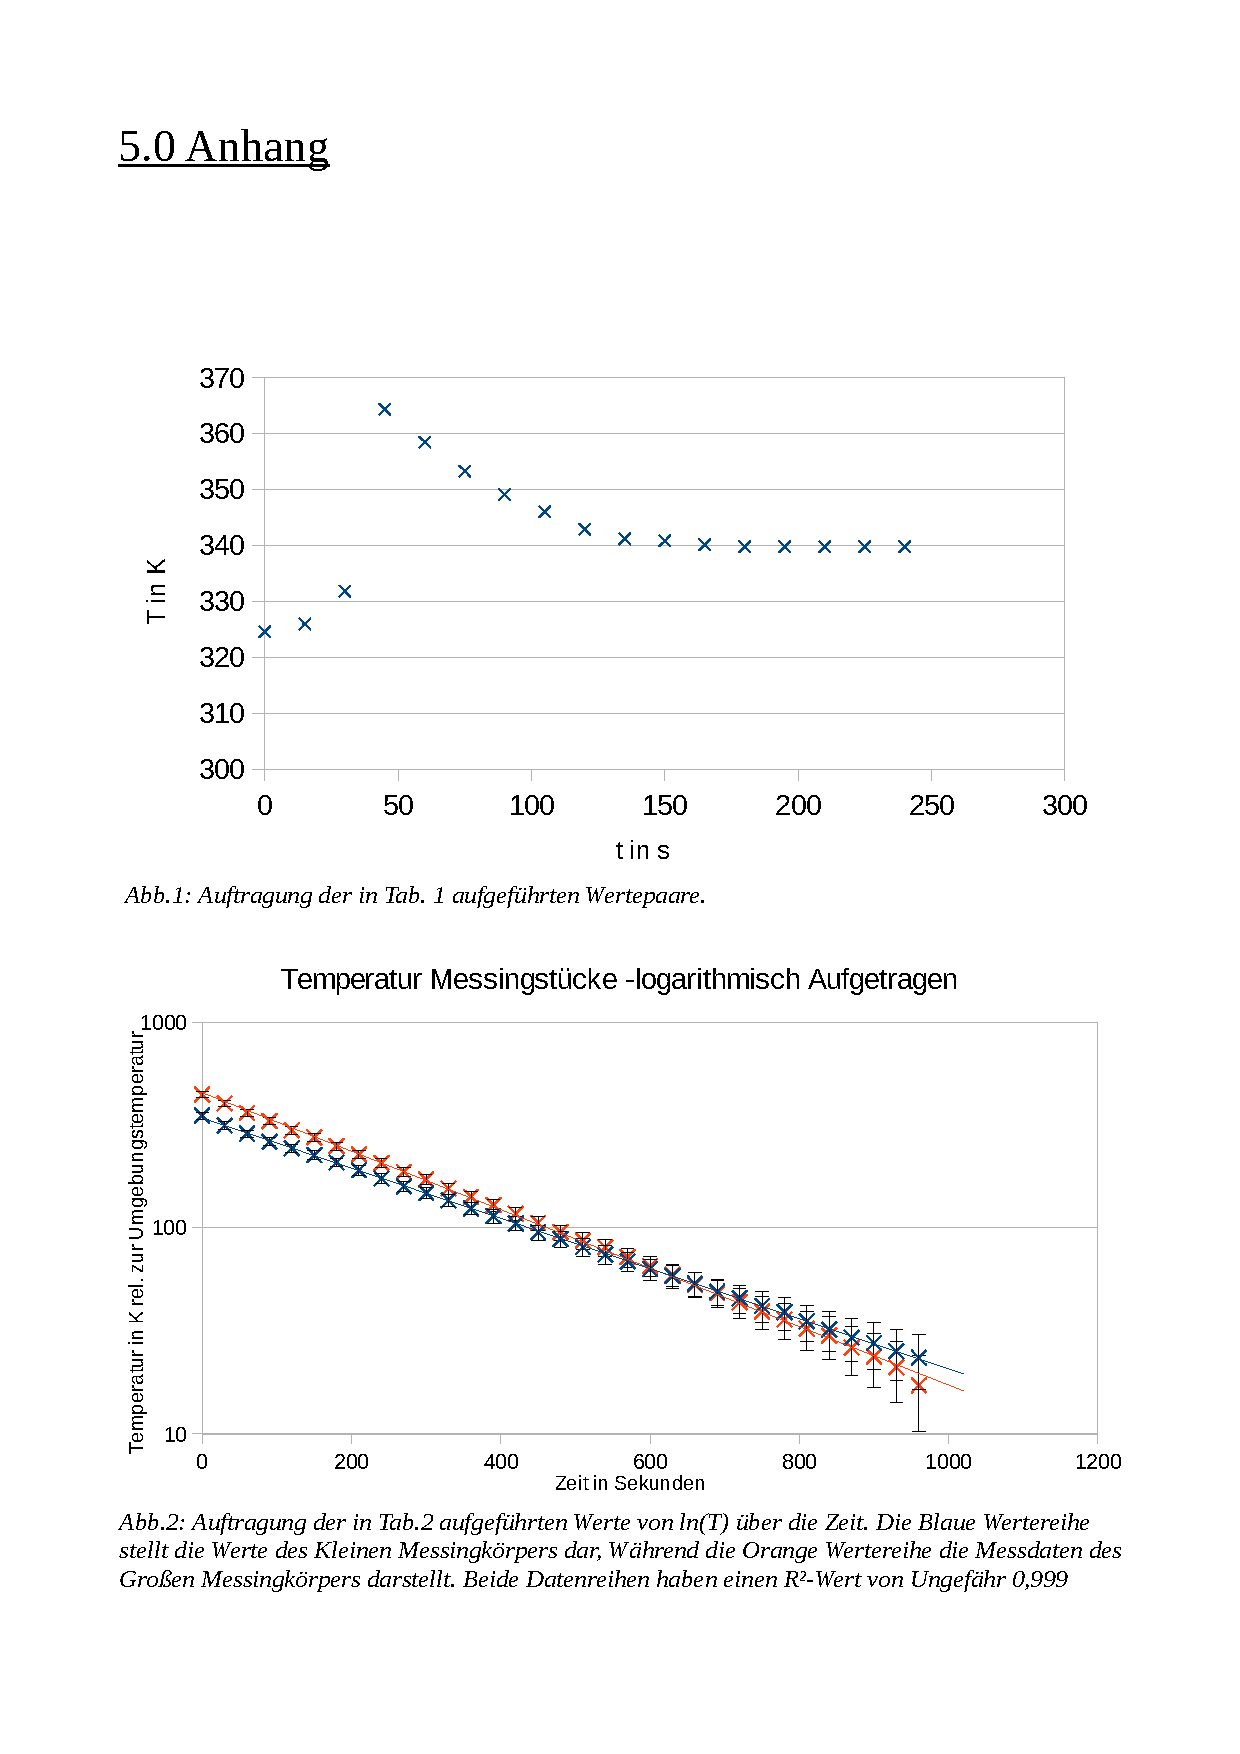
\includepdf{/home/janosch/Schreibtisch/UHB/SEM2/PHY-B/Praktikum/[1]T5/Diagramme}
\end{document}